\chapter{Kontekst}
\label{ch:kontekst}

Sedaj smo pripravili korpus in čas je, da ga prikažemo. En način prikaza je oblak besed, ki ga že poznamo. \textit{Word Cloud} nam prikaže pogostost besed. Pogostejša kot je beseda, z večjimi črkami bo zapisana.\marginnote{Vizualizacije v Orangeu so narejene tako, da podpirajo izbor podmnožic. Odkrivanje zanimivih podmnožic in raziskovanje njihovih podobnosti je ključni del odkrivanja znanj iz podatkov.}

Še vedno pa ne vemo, kako se besede uporabljajo v besedilu. Na primer ‘oh’ je lahko maločrkovna verzija besede OH (kemijska spojina hidroksid), preprost vzklik ‘Oh!’ ali pa kratica za ameriško zvezno državo Ohio.

Da bi preverili kontekst posamezne besede, lahko uporabimo gradnik Concordance. \textit{Concordance} na pokaže besedilo okrog izbrane besede.
Pozvežite Concordance z gradnikom \textit{Corpus}. Tako Concordance dobi vhodno besedilo. Besedo lahko poiščemo z iskalnikom na vrhu gradnika ali pa jo izberemo v gradniku \textit{Word Cloud}.

\begin{figure*}[h]
  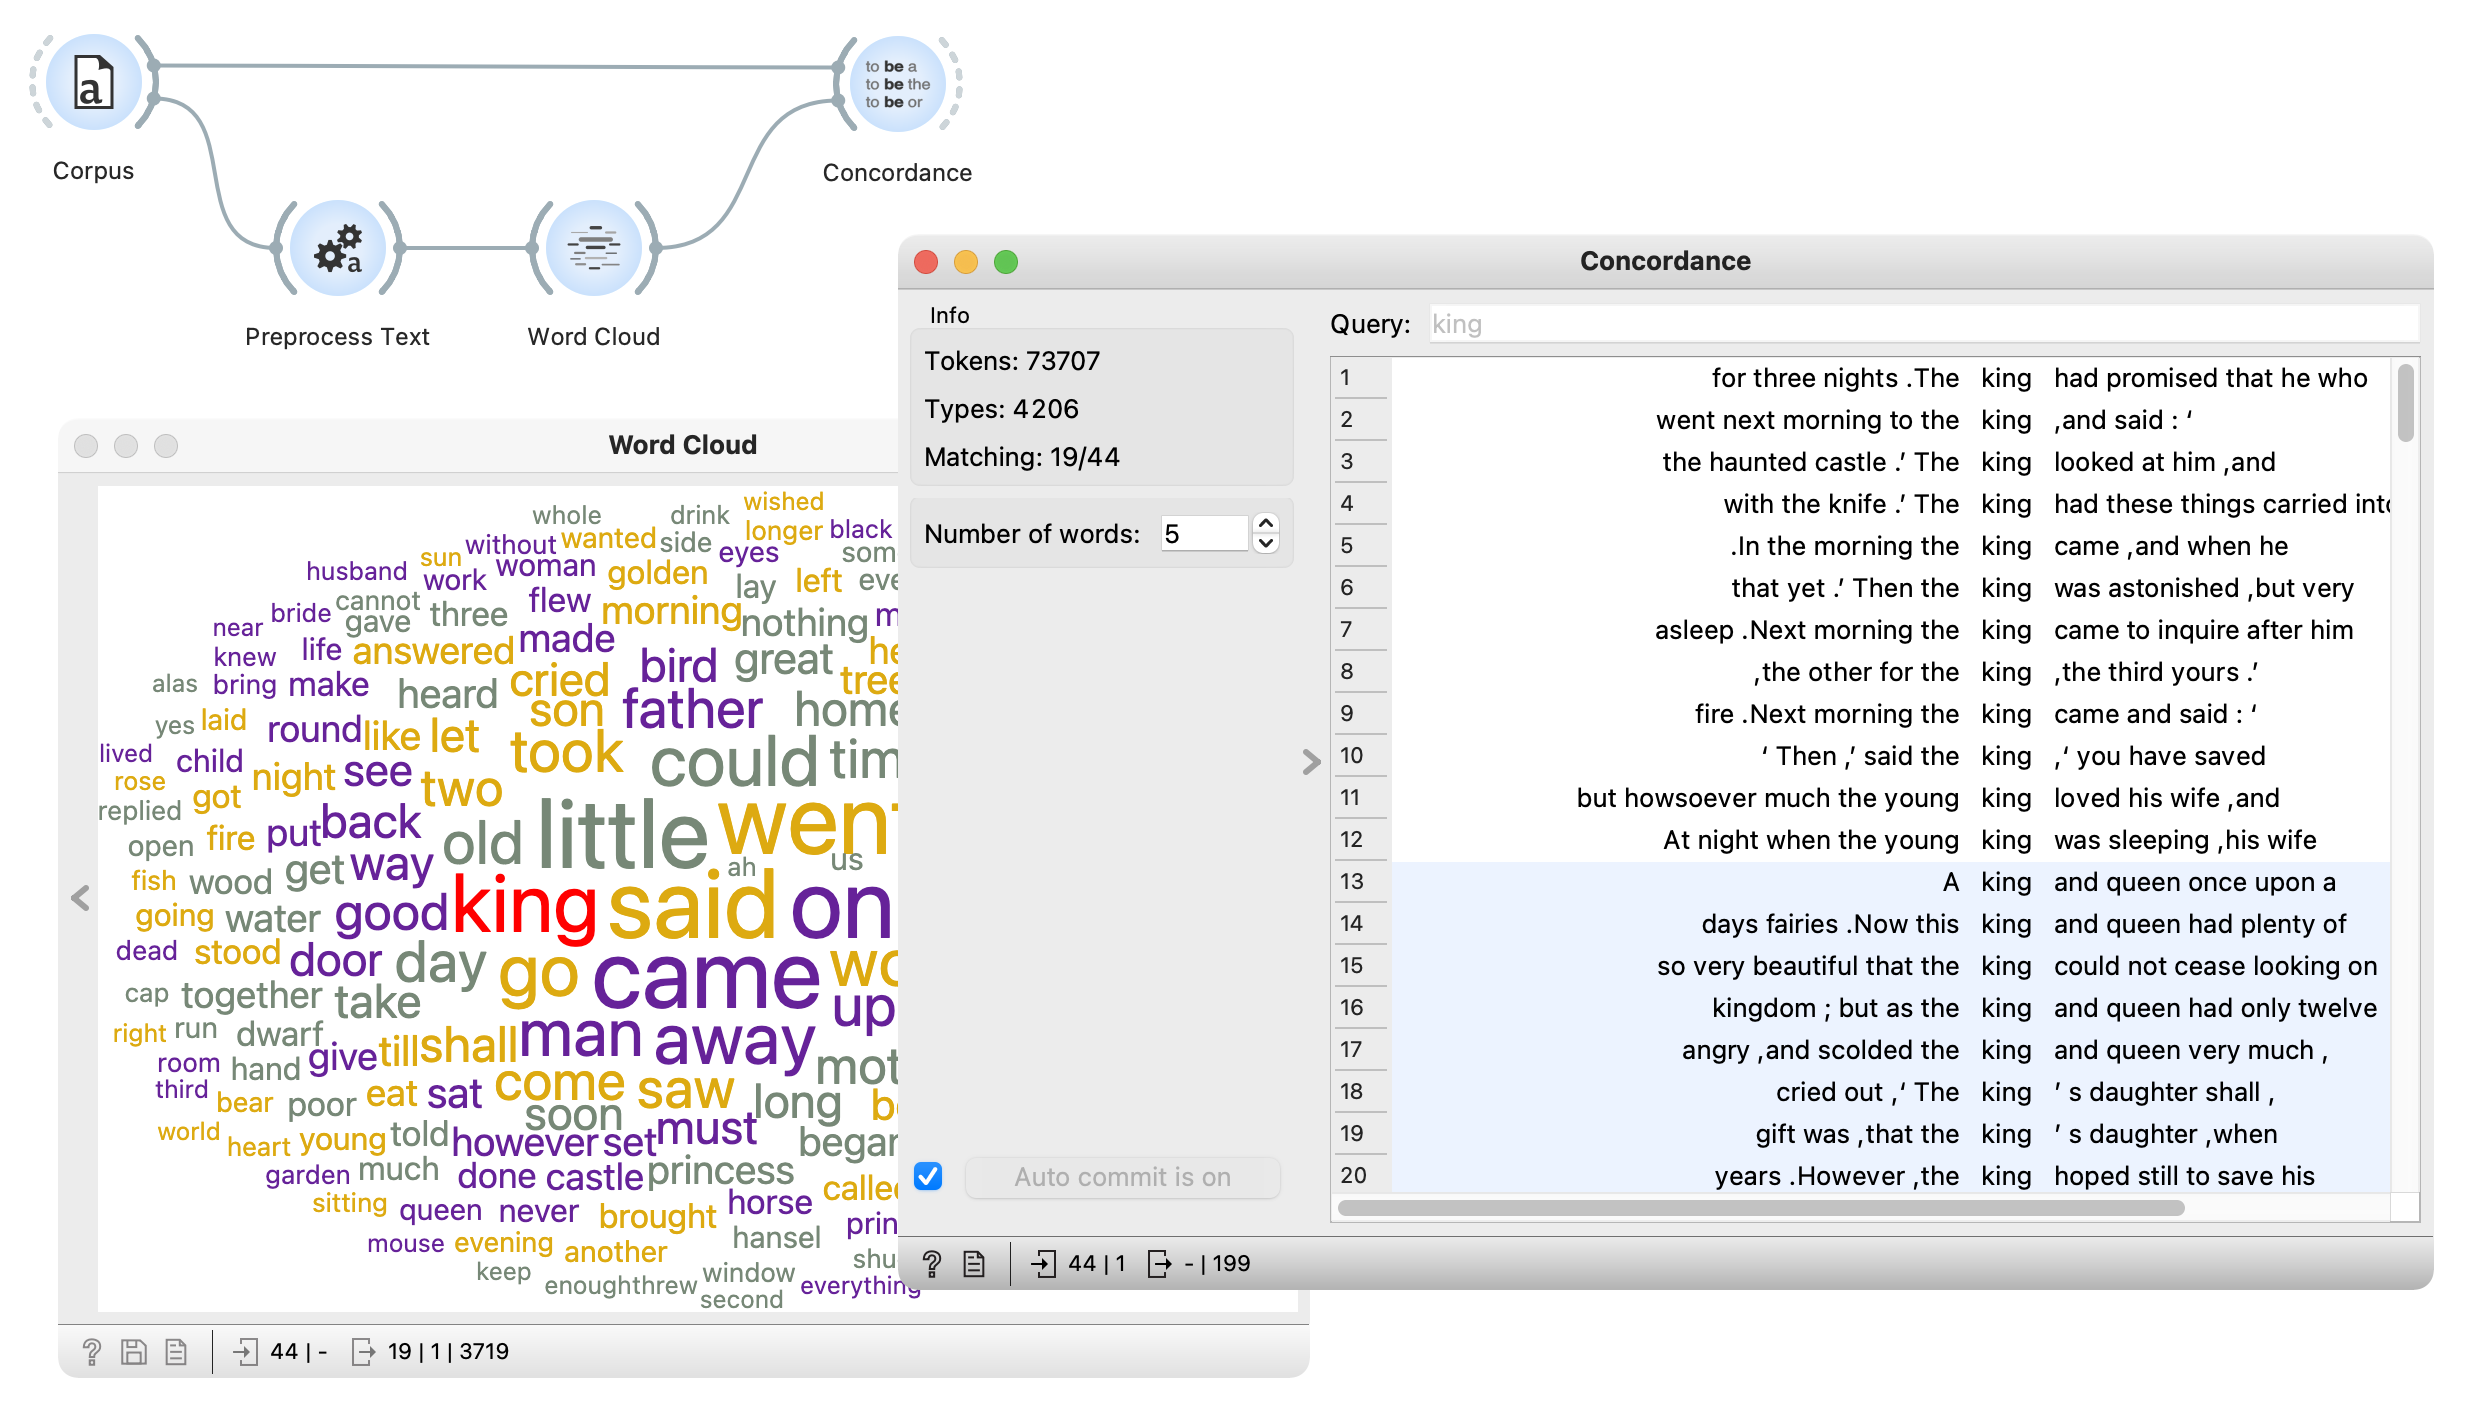
\includegraphics[width=\linewidth]{kontekst.png}%
  \caption{Dokumente, ki vsebujejo izbrano besedo, si pogledamo tako, da izberemo dokumente v gradniku Concordance in jih pošljemo v Corpus Viewer za podrobnejšo analizo. }
  \label{fig:003-kontekst}
\end{figure*}

V tem primeru smo izbrali besedo ``king'' v oblaku besed in preverili njen kontekst v gradniku Concordance.